%!TEX encoding = UTF-8 Unicode

\section{ウェブインタフェースを介したHPCシステム利用環境}

\subsection{緒言}
前章では,本研究の関連研究について述べた.本章では,ウェブインタフェースを介したHPCシステム利用環境の提案手法について説明し,その実装を行う.はじめに,提案手法の概要を説明する.その後,実装の概要,具体的な実装の手順について説明する.\par

\subsection{提案手法}
本研究の目的は,HPC利用環境をウェブインタフェースに提供する機能 (ウェブ機能)と,ジョブスケジューラ間の差異を抽象化する機能 (スケジューラ抽象化機能)に切り分け,それぞれ独立に保守できる構成を実現することである.このために,本研究ではウェブ機能からは統一的にシステムを利用し,スケジューラ抽象化機能でシステム間の差異を埋める構成の利用環境を提案する.\par
この提案手法の模式図を図\ref{fig6}に示す.ウェブ機能では,ユーザはウェブ機能のみとやり取りを行い,ユーザ情報を管理する外部の認証用ディレクトリを用いて安全にHPCシステムを利用することができる.スケジューラ抽象化では,ウェブ機能から得られた様々なジョブスケジューラに対する要求をスケジューラ抽象化機能が受け取り,処理を行う.この実現のためには,ウェブ機能とスケジューラ抽象化機能を連携させる必要があることから,両者間に求められる情報のやり取りを整理し,適切な実装方法を検討する.\par

\begin{figure}[tb]
    \centering
    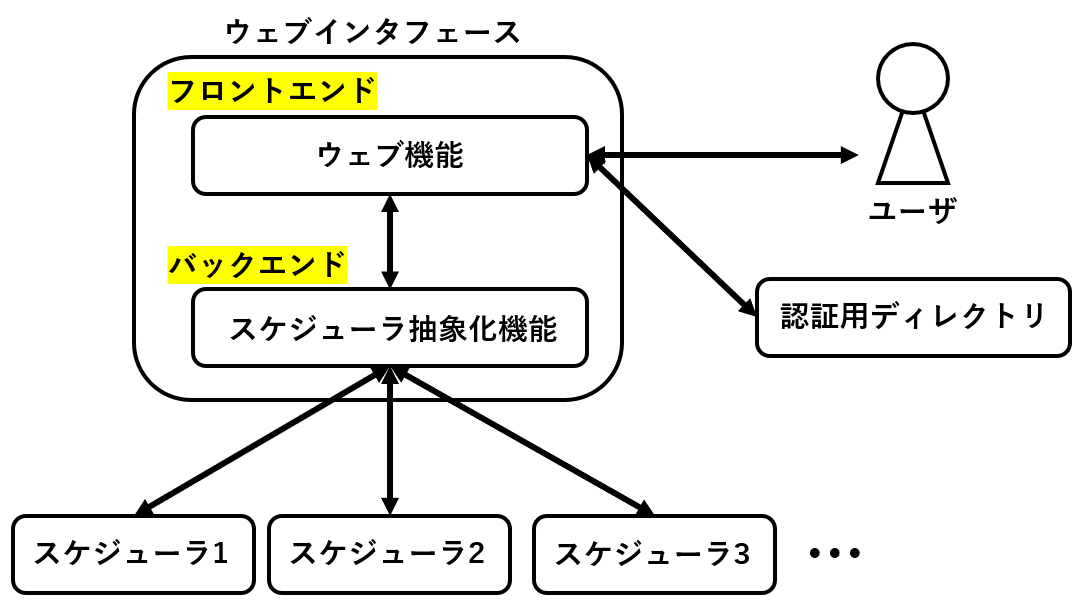
\includegraphics[width=120mm]{./fig/proposed_method.png}
    \caption{提案手法の模式図}
    \label{fig6}
\end{figure}

\subsection{実装}
\subsubsection{実装の概要}
ウェブ機能とスケジューラ抽象化機能をそれぞれ独立に実装し,連携させることでウェブインタフェースを介して様々なシステムを統一的に利用できる環境を実現する.そのために,ウェブ機能の基盤としてOODを利用する.さらに,スケジューラ抽象化機能の基盤としてPSI/J\cite{cite5}と呼ばれるPythonライブラリを利用する.PSI/Jは複数のジョブスケジューラを統一的に取り扱うことを可能とするライブラリである.両者を組み合わせることで提案手法の実装を行う.\par
本研究では,東北大学のスーパーコンピュータ「AOBA」\cite{aoba}で運用されているジョブスケジューラ (NEC Network QueuingSystem V, NQSV) \cite{nqsv_scheduler}がOODに対応していないという事実に着目して,NQSVをスケジューラ抽象化機能側に実装することと,それをウェブ機能側から利用できることを検証する.実装環境として,OOD用のホストサーバとスーパーコンピュータAOBAを模したHPCクラスタ (疑似AOBAクラスタ)を考える.疑似AOBAクラスタの模式図を図\ref{fig7}に示す.OOD用のホストサーバでは,OODの動作が保証されているUbuntu20.04 LSTをOSとして用いる.疑似AOBAクラスタは,マスターノードと二つのワーカーノードから構成される小規模なクラスタであり,AOBAと同様にNQSVがジョブスケジューラとして利用されている.疑似AOBAクラスタではNQSVの動作確認が行われているCentOS7を用いる\cite{nqsv_introduction}.本研究の実装では,公式が推奨しているLDAPサーバを用いた「DexとのOpenIDコネクト」を利用して認証を行う\cite{cite7}\cite{cite8}.OpenIDコネクトとはユーザ認証用のプロトコルのことを指し,DexはOpenIDコネクト認証プロバイダーである.LDAPとは,ユーザIDやパスワードの管理を行うディレクトリサービスの維持およびアクセスを行うプロトコルである.また,LDAPサーバとは,LDAPに基づいてディレクトリサービスを提供するサーバのことである.\par

\begin{figure}[tb]
    \centering
    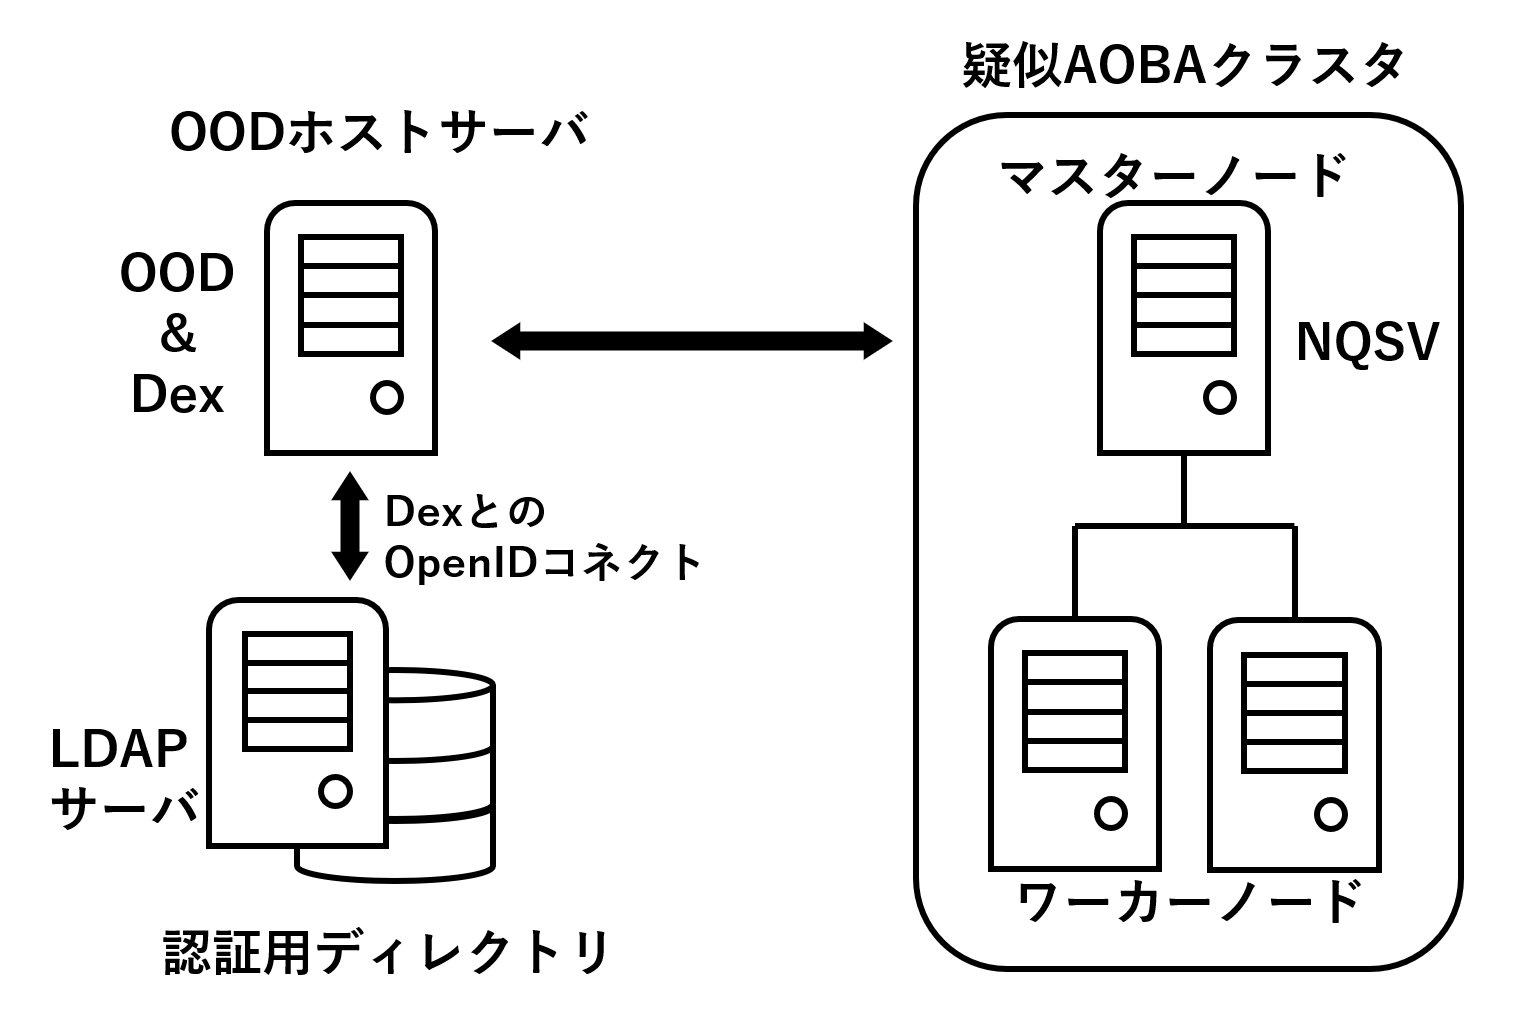
\includegraphics[width=120mm]{./fig/environment.png}
    \caption{実装環境}
    \label{fig7}
\end{figure}


\subsubsection{スケジューラ抽象化機能とNQSVの連携}
スケジューラ抽象化機能とNQSVの連携を考える.スケジューラ抽象化機能の基盤であるPSI/Jは,ジョブの情報を格納するJobクラスとジョブの投入や削除などのメソッドをジョブスケジューラごとに再定義しているJobExecutorクラスにより構成されている.本研究では新たにNQSV用のJobExecutorクラスを作成し,ジョブの投入,削除,ジョブの状態確認を行うための3つのメソッドを実装する.\par
はじめに,ジョブの投入を行うメソッドを実装する.
続いて,ジョブの削除を行うメソッドを実装する.
最後に,ジョブの状態確認を行うメソッドを実装する.PSI/Jが対応している他のジョブスケジューラ (Slurm,PBS Pro,LSF,Flux,Cobalt)はジョブの終了後にジョブの状態 (COMPLETED,CANCELED,FAILED)をコマンドの出力結果から確認できる.しかし,NQSVではジョブの終了後にCOMPLETED,CANCELED,FAILEDの状態を確認できない.そのため,NQSVに対応するためには,ジョブの投入,ジョブの削除,および待機中のジョブの存在確認に基づいてジョブの状態をPSI/J側で把握する必要がある.この機能を実現するため,本研究の実装ではジョブが投入された後にジョブキューからジョブが無くなった際に,そのジョブの状態をCOMPLETEDに変更する.また,ジョブが削除された際には,そのジョブの状態をCANCELEDに変更する.それ以外にジョブキューの状態をコマンドを用いて定期的に確認し,出力結果に応じてQUEUEDあるいはACTIVEという状態にする.\par
具体的な実装をコード\ref{get_status_now}に示す.JobExecutorクラス内で定義されているget\_status\_nowメソッドはJobクラスのインスタンスを引数にとり,ジョブの状態を保持するJobStatusクラスを返り値に持つ (30行目).引数から受け取ったJobクラスのインスタンス変数job.native\_idからジョブのIDを抽出し,string型変数native\_idsに代入する (31行目).各ジョブスケジューラごとに指定されているジョブの状態確認コマンドをジョブIDを指定して投げる.本研究では,NQSV用のコマンドとして「qstat -F rid,stt -n -l native\_ids」を用いて,指定したIDのジョブのIDと状態を返すコマンドオプションを利用する (32~34行目)\cite{nqsv_reference}.コマンドの出力は行ごとにList型変数のlinesに代入され,中身をforループでまわす (36~38行目).lines変数の中身は空白区切りのstring型としてcolsに代入される.指定したIDのジョブがジョブキューにない場合は,ジョブのIDとジョブの状態ではなく「Batch Request: ジョブID does not exist on クラスタのホスト名.」という出力が変数colsに代入されるため,条件文「len(cols)==8」が真であれば指定したIDのジョブがジョブキューにないということがわかる.そのため,条件文が真であり,cancel時に立つcancel\_fragが立っていればジョブキュー内にジョブがなく,ジョブの削除が正常に行われている状態であるため,ジョブの状態をCANCELEDにする (43~51行目).一方,条件文が真であり,cancel\_fragが立っていない場合は,ジョブキュー内部にジョブがないが,ジョブの削除が行われていないので,ジョブの状態をCOMPLETEDにする (53~61行目).また,ジョブの投入時に立つsubmit\_fragが立っていない場合はそもそもジョブの投入が成功していないのでジョブの状態をFAILEDにする (63~71行目).以上の三つの場合分けにおいて,「Batch Request: ジョブID does not exist on クラスタのホスト名.」という出力からジョブIDのみを抽出して,ジョブIDごとにlist型変数rを用意してJobStatusクラスのジョブの状態情報を代入する.また,前述した3種類の場合分けのどれにも値しない場合は,ジョブキュー内にジョブが存在する場合であり,ジョブIDとジョブの状態が変数colsに代入される.ここで出力されているジョブの状態はNQSVによって定められた状態名でありジョブキューに投入され,実行待ちである状態はQUE,ジョブが実行されている状態はRUNなど固有の名称が定められている.これらの固有のジョブ状態名からPSI/Jで用いる各ジョブスケジューラで共通の状態名に変換するために,\_STATE\_MAPと\_get\_stateメソッドを用いる.なお,他のジョブスケジューラではジョブ状態の詳細メッセージが出力される場合があるが,NQSVには詳細メッセージの出力機能がないためmessage変数はNoneとしている.\par
このようにPSI/J自身がジョブの状態を管理することにより,さらに広い範囲のジョブスケジューラに対応することができることから,ジョブスケジューラ抽象化機能の汎用性を高めることができたといえる.\par

\begin{lstlisting}[caption=ジョブの状態取得メソッド, label=get_status_now]

class NQSVJobExecutor(BatchSchedulerExecutor):

    _STATE_MAP = {
        'QUE': JobState.QUEUED,
        'RUN': JobState.ACTIVE,
        'WAT': JobState.QUEUED,
        'HLD': JobState.QUEUED,
        'SUS': JobState.QUEUED,
        'ARI': JobState.QUEUED,
        'TRS': JobState.QUEUED,
        'EXT': JobState.ACTIVE,
        'PRR': JobState.QUEUED,
        'POR': JobState.ACTIVE,
        'MIG': JobState.QUEUED,
        'STG': JobState.QUEUED, 
    }

    def get_status_command(self, native_ids: Collection[str]) -> List[str]:
    return ['qstat', '-F', 'rid,stt', '-n', '-l'] + list(native_ids) 

    def get_status_now(self, job: Job) -> Job.status:
        native_ids = ''.join(str(job.native_id))
        command = ['qstat', '-F', 'rid,stt', '-n', '-l', native_ids]
        out = 
        subprocess.run(command, capture_output=True, text=True).stdout
        r = {}
        lines = iter(out.split('\n'))

        for line in lines:
            if not line:
                continue
            cols = line.split()

            if(len(cols) == 8 and self.cancel_frag):
                s = cols[2]
                native_id = ""
                for char in s:
                    if char.isdigit():
                        native_id += char
                state = JobState.CANCELED
                r[native_id] = JobStatus(state=state, message=None)
                return r[native_id]
            
            elif(len(cols) == 8 and not(self.cancel_frag)):
                s = cols[2]
                native_id = ""
                for char in s:
                    if char.isdigit():
                        native_id += char
                state = JobState.COMPLETED
                r[native_id] = JobStatus(state=state, message=None)
                return r[native_id]

            elif(not(self.submit_frag)):
                s = cols[2]
                native_id = ""
                for char in s:
                    if char.isdigit():
                        native_id += char
                state = JobState.FAILED
                r[native_id] = JobStatus(state=state, message=None)
                return r[native_id]
            
            else:
                assert len(cols) == 2
                match = re.search(r'\b(\d+)\b', cols[0])
                native_id = match.group(1) if match else None
                native_state = cols[1]
                state = self._get_state(native_state)
                msg = None
                r[native_id] = JobStatus(state=state, message=msg)
                return r[native_id]
    
    def _get_messsage(*args, **kwargs):  
    return None
    
    def _get_state(self, state: str) -> JobState: 
        assert state in NQSVJobExecutor._STATE_MAP
        return NQSVJobExecutor._STATE_MAP[state]
\end{lstlisting}


\subsubsection{ウェブ機能とスケジューラ抽象化機能との連携}
続いて,ウェブ機能側であるOOD側からスケジューラ機能を用いることを考える.実装における問題点として,OODがRubyで実装されていることに対して,PSI/JはPythonで実装されているという点が挙げられる\cite{cite9}\cite{cite10}.そのため,Rubyスクリプト上でPythonライブラリを使用する必要がある.本実装ではPSI/Jを経由する際のオーバヘッドが小さく,単純な実装であるため,PSI/Jを用いたジョブの管理のためのPythonスクリプトをシェルを経由してRubyスクリプト上で直接実行する.この実装により,ウェブ機能としてOODを用い,スケジューラ抽象化機能であるPSI/Jを経由して,指定したジョブスケジューラにジョブの投入や削除を行うことができる.また,PSI/Jを仲介することで,OODが未対応であったNQSVでのジョブ管理をOOD上から操作することを実現している.\par
実装をコード\ref{psij_to_ood}に示す.PSI/Jと連携するためのアダプタファイルはOodCore/Job/Adapters空間内で定義され,AdapterスーパークラスのサブクラスとしてPSIJクラスを定義する.図\ref{設定ファイル}にはOODとPSI/Jを接続するための設定ファイルpsij.ymlの中身を示す.設定ファイルには,OODからログインを行う際のホスト名,選択するAdapter名,PSI/Jで用いるJobExecutorクラス名,バイナリファイルのパスと用いるジョブスケジューラの設定ファイルのパス,ジョブを投入するHPCクラスタのホスト名を設定する.initializeメソッド内では,設定ファイルpsij.ymlから与えられた情報をそれぞれインスタンス変数に代入する.submitメソッドでは,引数にジョブスクリプトの中身をとり,返り値に投入したジョブのIDを渡す.与えらえれたジョブスクリプトは一時的なジョブスクリプト保管用のディレクトリに保管され,scpコマンドを用いて,ユーザのホームディレクトリにPSI/Jを用いたジョブ投入用のpythonスクリプトsubmit\_script.pyを転送する.その後,ジョブ投入先のホストでJobExecutorと投入するジョブのパスを指定してsubmit\_script.pyを実行することでジョブが選択したホストに投入されるようになる.\par
実際に,OODのJob Composer画面からジョブの投入を試みる.ジョブを作成する際にクラスタ選択で「psij」を設定することで,PSI/Jを経由してSlurmクラスタやNQSVクラスタなど任意のHPCシステムにジョブを投入できていることが確認できた.\par

\begin{lstlisting}[caption=PSI/JとOODの連携, label=psij_to_ood]

class PSIJ < Adapter
  class Batch
    def initialize(cluster: nil, bin: nil, conf: nil, bin_overrides: {}, 
              submit_host: "", strict_host_checking: true, executor: nil)
      @cluster              = cluster && cluster.to_s
      @conf                 = conf    && Pathname.new(conf.to_s)
      @bin                  = Pathname.new(bin.to_s)
      @bin_overrides        = bin_overrides
      @submit_host          = submit_host.to_s
      @strict_host_checking = strict_host_checking
      @executor             = executor
    end

  def submit(script, after: [], afterok: [], afternotok: [], afterany: [])
    job_path = "/Temporary/Path/to/run.sh" 
    file = File.open(job_path, "w")
    file.puts(script.content.to_s)
    file.close
    scp_command = "sshpass -p 'password' scp /Path/to/submit_script.py 
                  username@#{@psij.submit_host}:/Path/to/submit_script.py"
    system(scp_command)
    psij_submit = 
    "python3 /Path/to/submit_script.py" 
                          + " " + @psij.executor + " " + job_path
    ssh_submit = 
    "sshpass -p 'password' 
                  ssh username@#{@psij.submit_host} '#{psij_submit}'"
    o, e, s = Open3.capture3(ssh_submit)
    return o
  end
  
  def delete(id)
    ids = id.to_s
    scp_command = "sshpass -p 'password' scp /Path/to/delete_script.py 
                  username@#{@psij.submit_host}:/Path/to/delete_script.py"
    system(scp_command)
    psij_delete = 
    "python3 /ood_tmp/delete_script.py" + " " + @psij.executor + " " + ids
    ssh_delete = 
    "sshpass -p 'password' 
                  ssh username@#{@psij.submit_host} '#{psij_delete}'"
    system(ssh_delete)
  end

\end{lstlisting}

\begin{figure}[tb]
    \centering
    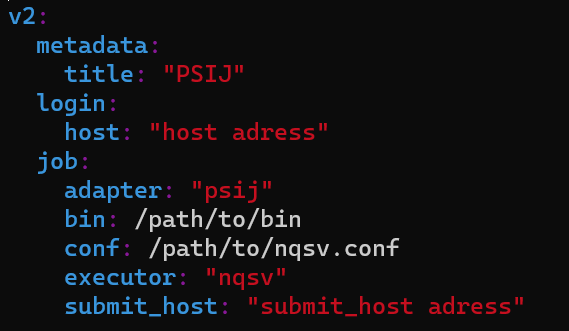
\includegraphics[width=120mm]{./fig/PSIJ.yml.png}
    \caption{OODとPSI/Jの接続ファイル}
    \label{設定ファイル}
\end{figure}

\subsection{結言}
本章では,ウェブインタフェースを介したHPCシステム利用環境の提案手法について説明し,その実装を行った.はじめに,提案手法の概要を説明した.その後,実装の概要,具体的な実装の手順について説明した.次章では,本章で実装した提案手法の性能評価を行い,提案手法の有用性を考察する.